% !TEX root = ../main_zh.tex
\chapter{国民收入核算}
\label{ch:accounts}

在解释经济为何繁荣与萧条、增长与停滞之前，我们首先需要一套度量经济产出的办法。宏观经济学研究的是总量——总产出、总收入、总支出——而一个总量的价值，全在于代表它的那个数字。国民收入核算正是这样一套定义与恒等式的体系，它把千百万家庭与厂商纷繁的活动，浓缩成寥寥几个可以度量的数量。它之于宏观经济学家，犹如财务报表之于企业：单看枯燥乏味，却是后续一切分析不可或缺的根基。

核算的核心对象是国内生产总值（GDP），即一个经济体在一段时期内所生产的一切产品的市场价值。本章的大部分篇幅，都是在细致拆解这一句话，因为其中几乎每一个限定词都是经过深思熟虑的选择，并各有其后果。随后我们会看到，同一个总量可以由三条不同的路径得到——按生产计、按收入计、或按支出计——而这三条路径殊途同归，并不是有待证明的定理，而是核算体系本身内建的恒等关系。从支出路径，我们读出对需求的著名分解：消费、投资、政府购买与净出口；从收入路径，读出从 GDP 一路细化到个人可支配收入的链条；从金融市场，读出把家庭储蓄、政府赤字与贸易差额捆在一起的储蓄—投资恒等式。本章最后讨论两个实务问题：产出如何按产业归类，以及在官方数据发布的间隙，分析者如何对 GDP 进行旁敲侧击的估计。

有一句告诫贯穿始终：没有任何单一指标能概括整个国民经济，而 GDP 尤其是为\emph{可度量}而设计的，并不是衡量福利的完整标尺。分清它计入了什么、又遗漏了什么，这场仗就赢了一半。

\section{国内生产总值}

\defn{国内生产总值}{
\emph{国内生产总值（GDP）}是指在给定时期内，一个经济体在其地理疆界之内所生产的全部最终产品和服务的市场价值。
}

慢慢读，这条定义包含了五个限定词，每一个都排除了某些东西。我们逐一来看。

\subsection{五个限定词}

\textbf{（1）给定时期——GDP 是一个流量。} GDP 总是针对一段时间报告，通常是一个季度或一年；全球的任何国家都有年度和季度 GDP。正因为它是在\emph{一段时间内}度量的，所以 GDP 是一个\emph{流量}（flow），而不是\emph{存量}（stock）。流量是指在一段时间内测度的数量，存量是指在某个时点上测度的数量。这一区分绝非咬文嚼字——它是宏观经济学中最常见的混淆来源，我们应当养成习惯：对每一个宏观变量都先问一句，它是存量还是流量。

举例来说，财富水平就是一个存量：在这一时刻，经济中总的财富水平是可以测度的。而 GDP 是一个流量，二者并不是一回事。2010 年前后中国 GDP 超过了日本，只能说明从那一年起，中国每一年比日本生产了更多的产品和服务；它并不意味着中国累积的\emph{财富}水平超过了日本——后者很可能尚未发生。

\rmkb[收入、财富，以及金融为何相互抵消]{把三组相关的流量与存量分开来看会很有帮助。\emph{收入}（流量）等于劳动收入——工资、奖金——加上资本收入——金融资产的\emph{收益}，例如股权分红、利息，但\emph{并不是}资本存量本身。\emph{财富}（存量）则是实物资产与金融资产之和。宏观经济学主要关心收入；财富更多是个人才关心的问题。还要注意，对整个社会而言，金融资产并不是净财富：每一项金融资产都是某个主体对另一个主体的权益要求凭证，在全社会加总时这些要求相互抵消。正因如此，宏观核算可以将其忽略而账目仍然平衡。}

\rmkb[何时会出现月度 GDP]{通常没有月度 GDP，因为数据来不及处理。但在特殊情形下，当局也会估算它：2022 年疫情扰动期间，中国密切跟踪月度数据，以制定增长目标、稳定预期——2022 年 4 月约为 $-2.2\%$，5 月约为 $-0.1\%$，6 月约为 $+4\%$，合计起来二季度约为 $+0.5\%$。在中国，每月 16—20 日左右公布按收入法初步核算的 GDP；月度的实体经济数据基本上都是\emph{名义值}，因为来不及做价格平减。完整的支出法年度核算——其中包含居民消费和政府消费的比重——则要等到次年的五六月份才公布。}

\textbf{（2）市场价值。}由于 GDP 要把苹果、理发与软件统统加在一起，它就必须用一个共同的单位来给一切定价，而这个单位就是市场价格。依赖市场价格有一个直接的推论：那些从不在市场上交易的东西没有可观察的价格，因而原则上难以核算——自给自足的自然经济成分、家庭家务劳动以及非法交易都在其列。关键在于，产品或服务\emph{能且会}以市场价格易手，而不是说每一单位都必须真的发生过一次交易（下文将讨论的存货，就是先被计入、后才售出的产出）。

\textbf{（3）地理范围——“国内”。} GDP 是按\emph{疆界}定义的。中国的 GDP 涵盖在中国境内进行的生产，不论生产者是中国国民还是外国人。在全球化时代，这是自然的选择，也与“地方政策须与当地条件相适配”的逻辑一致；我们将在下文把它与按国民计的口径（GNP）作对比。

\textbf{（4）最终品，而非中间品。}一件产品究竟是\emph{最终品}还是\emph{中间品}，取决于它的用途。被用作进一步生产之投入而消耗掉的，是中间品；为消费或投资而购买的，是最终品。GDP 只核算最终品。这样做是为了避免\emph{重复计算}：如果把面粉和蛋糕都算上，面粉就被计了两次。注意，同一件实物产品可以是其一，也可以是其二，全看用途——家庭买来在家做蛋糕的面粉是最终品，而烘焙店买来做蛋糕出售的面粉则是中间品。

\textbf{（5）市场销售或推算的产出。} GDP 核算的是被生产并在市场上销售的东西，外加少数几样并非真的售出、却\emph{理应}按市场价值估算的东西，即通过推算（imputation）计入。最典型的例子是自有住房的居民“向自己购买”的住房服务：核算时会加上一笔推算租金。（把买房的价格计入 GDP，与把它日后产生的住房服务流计入 GDP，二者并不矛盾——它们是不同的东西，下文讨论投资时会说明。）

\subsection{何者计入、何者不计}

五个限定词已能处理大多数情形，但边界仍足够微妙，值得把那些标准的处理口径集中列在一处。其组织原则很简单：\emph{GDP 只把新创造的价值计入一次}。

\rmkb[GDP 计入与否的边界情形]{
\begin{itemize}
    \item \emph{没有新创造，就不计入。}政府税收和转移支付不计入 GDP——它们只是把既有资金重新分配。（政府雇员的\emph{工资}\emph{要}计入 GDP，因为那是对其所提供服务的报酬。）股票交易不计入 GDP，因为它只是所有权的转移、并无新增产出；交易的印花税不计入 GDP，因为那只是把一部分资金转移给政府；但\emph{佣金}要计入 GDP，因为经纪是一项被生产出来的服务。
    \item \emph{只计新创造的那一部分。}新房成交价并非全部计入 GDP，因为其中一部分是地价。只有土地上新建建筑的价值才计入。购房时缴给政府的税款不计入。
    \item \emph{存货作为投资计入。}今年生产、尚未售出的产品仍是今年的产出，无论它最终何时成交。从支出口径看，当存货品日后被卖出时，消费（或投资）支出上升，而存货同时等额下降，二者相抵。
    \item \emph{推算价值。}未在市场上销售、但概念上可市场化的产出，会经推算后计入——自有住房服务是标准情形。
    \item \emph{研发如今算作投资。}研发支出过去被视为生产过程的中间投入，如今计为投资。
    \item \emph{服务按价格而非质量计价。}一项服务按其价格计入，与它质量好坏无关。
    \item \emph{防御性支出会虚增 GDP。}仅仅为抵消某种负外部性而发生的活动同样被计入，从而高估了真实产出与福利。倘若某企业在生产时造成污染，它的产出本身计入了 GDP，事后的治理清污又再次计入 GDP——GDP 于是被二次虚增。
\end{itemize}
}

最后一点是最尖锐的提醒：GDP 是一笔产出的清点，而不是福利的指数。这条定义的选取，一半是为了它的含义，一半是为了它的可度量性，结果便是它有意地把大量价值留在了账外。

\subsection{从国内到国民：GNP 与 GNI}

地理这一限定词有一位天然的“近亲”。GDP 把边界划在一片\emph{疆土}周围，国民生产总值则把边界划在一群\emph{国民}周围。

\defn{国民生产总值}{
\emph{国民生产总值（GNP）}是指在给定时期内，一个国家的\emph{国民}所生产的全部最终产品和服务的市场价值，无论他们在世界何处进行生产。
}

两个口径只在“计入哪些人”上有所不同，并由一个干净的调整项相联系：
\[
\mathrm{GNP} = \mathrm{GDP} + \pr{\text{本国人在境外的生产}} - \pr{\text{外国人在境内的生产}}.
\]
对一个大型经济体而言，GDP 与 GNP 之间的差距很小。世界银行用人均 GNP——如今改称为国民总收入（GNI）——来衡量一国国民的富裕程度，把各经济体划分为低收入、中等收入和高收入；中国目前处于上中等收入水平。

\section{循环流转与基本恒等式}

为什么各种度量产出的方法会给出同一个答案？原因在于：一个主体的支出正是另一个主体的收入，经济中的各笔支付在一个闭环里彼此追逐。这个闭环就是\emph{循环流转}（circular flow），如图~\ref{fig:macro-1} 所示。

\begin{figure}[h]
\centering
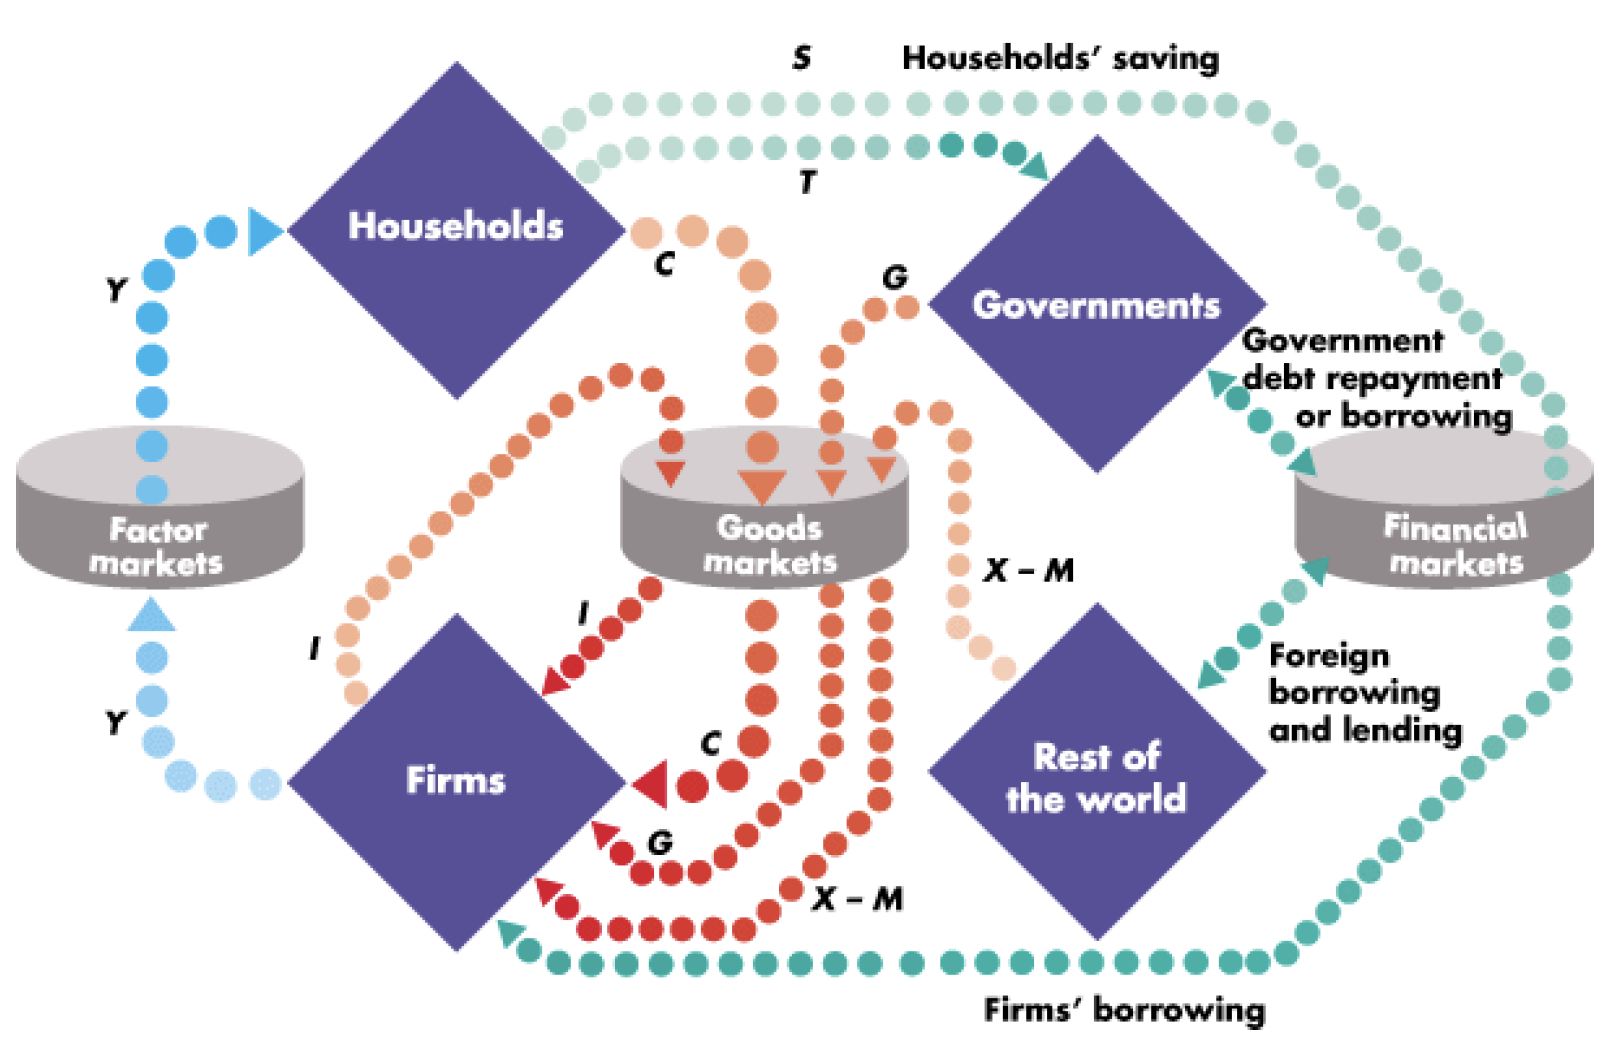
\includegraphics[width=\linewidth]{figures/fig1.png}
\caption{收入的循环流转：家庭、厂商、政府与世界其他地区跨越产品市场、要素市场与金融市场进行交易，从而使总收入等于总支出。}
\label{fig:macro-1}
\end{figure}

分析的核心在于\emph{家庭}。家庭是整个系统的枢纽，因为它既负责收入、也负责支出：广义地看，家庭是要素市场的供给方，也是产品市场的需求方。收入流向家庭，随后分散到消费 $C$、储蓄 $S$ 与税收 $T$，最终又以 $C$、$I$、$G$ 和净出口的形式重新表现为各项需求。

三个市场组织起整幅图景。\emph{产品市场}关联了主要的宏观经济主体——厂商、家庭、政府和世界其他地区。厂商是这个市场的供给方；需求来自家庭、政府和国外。\emph{要素市场}则闭合了这个循环：厂商在产品市场上赚得的收益，最终要回流去报偿生产要素，而这些要素的供给方——并因此获得相应收入——正是家庭。\emph{金融市场}把储蓄与投资联系起来，让经济得以向外国人“放贷”、使净出口得以发生，同时也与政府的财政紧密相连。

由于收入与支出本是同一笔支付从两侧看到的两面，总收入（AI）等于总支出（AE）：
\begin{equation}
\mathrm{AI} = Y = C + I + G + \pr{X - M} = \mathrm{AE}.
\label{eq:macro-identity}
\end{equation}
恒等式~\eqref{eq:macro-identity} 是\emph{事后}（ex post）成立的：按构造，已实现的收入恒等于已实现的支出。而总需求是\emph{事前}（ex ante）的概念——它是由意愿中的 $C + I + G + \mathrm{NX}$ 加总起来的、计划和打算进行的支出；短期波动恰恰起因于计划需求与已实现产出之间的背离。因此，分解式 $C + I + G + \mathrm{NX} = \mathrm{AD}$ 是一个短期对象，不断波动，且各项是按进行支出的\emph{主体}来划分的。

\subsection{拉动增长的三驾马车}

在像中国这样的经济体里，按主体划分支出会遇到麻烦：国家进行了大量投资，所有制又往往边界模糊——许多国有企业以混合甚至民营所有制运营，因此常常无法判断某笔支出究竟属于公共还是私人。补救之法是：不按\emph{谁}支出、而按支出的\emph{性质}来归类政府支出 $G$，把 $G$ 的每一部分重新归入消费或投资。政府\emph{消费}并入 $C$，政府\emph{投资}并入 $I$。（原则上 $I$ 还可再分为私人投资和政府投资，但统计上无法分开。）按性质划分后，\eqref{eq:macro-identity} 便坍缩为
\begin{equation}
\mathrm{GDP} = C + I + \mathrm{NX}.
\label{eq:macro-three-drivers}
\end{equation}
这三项就是著名的拉动经济增长的“三驾马车”：最终消费支出 $C$、资本形成总额 $I$，以及货物和服务的净出口 $\mathrm{NX} = X - M$。前两项之和 $C + I$ 是\emph{内需}；净出口是\emph{外需}；并能分别算出各自对一年增长的贡献率。

\section{通向同一总量的三条路径}

恒等式~\eqref{eq:macro-identity} 已经暗示，产出可以用不止一种方式来核算。标准的方法有三种，且按构造它们都得到同一个 GDP。

\subsection{生产法（增加值法）}

\defn{增加值}{
一个厂商的\emph{增加值}等于其销售额减去用于中间投入（原材料）的支出。按生产法核算的 GDP，就是把全经济所有生产性机构的增加值加总起来。
}

这种方法最直接地演绎了 GDP 的定义：增加值恰恰是厂商新创造的价值，把它加总起来就避免了对途经其间的中间品的重复计算。销售额、中间投入、增加值与 GDP 都是流量概念。

有一个细节值得强调：所减去的\emph{仅仅}是中间投入成本，而\emph{不包括}财务成本、用工成本或销售成本等（如工资、利息等支出）。生产法看的是\emph{生产}——也即生产性机构所创造的价值。它实际上把生产性机构当作 GDP 的来源，而不再单独去核算家庭通过提供要素所创造的价值；从效果上看，它是从整体上把握社会的生产过程。与之相对，若把全经济\emph{所有}的销售额加总起来，得到的是工农业总产值，其中的中间环节销售被重复计算了；中国征收的增值税，正是把这部分重复计算剥离了出去。

\subsection{收入法}

\defn{收入法}{
按\emph{收入法}核算的 GDP，是经济体中所有主体所赚取收入的加总，因为增加值终归会作为收入归于某个主体。
}

加总成 GDP 的收入包括：工资收入、利息收入（营运资本的回报）、税收收入，以及\emph{会计}利润——其中会计利润又包含经济利润和\emph{租金}两部分。租金这一项刻画的是：用于自己生产的机器设备，本可以拿到市场上租出去，自己使用它，实际上相当于自己生产、自己消费了这项租赁服务。存货也在此处计入，可理解为当年创造、来年创收的价值。

\subsection{支出法}

\defn{支出法}{
按\emph{支出法}核算的 GDP，是对最终产品和服务的支出之和：$C + I + G + (X-M)$。
}

它的焦点是产品市场。先把政府和进出口搁在一旁：产品市场上的每一件最终品，要么被家庭买走，要么被厂商买走。厂商作为资本品买走的机器设备是投资支出 $I$；其余几乎都是家庭的消费支出 $C$——只有一个标准的例外，即购房计入投资、而非消费。再把政府和进出口纳入进来，并不改变什么本质的东西；焦点始终落在产品市场上。按照惯例，家庭购买的物品——住房除外——其价值完全计在购买当期。

\state{三种方法，一个数字}{
生产、收入与支出，是从三个视角去观察同一个循环流转。生产中创造的增加值会作为收入归于某人，而那笔收入又会被支出。因此三种方法度量的是同一个 GDP，它们的相等是一条核算恒等式，而不是一项经验发现。
}

\section{金融市场核算与储蓄—投资恒等式}

金融市场连接起同样的四个主体——家庭、政府、厂商和外国人。家庭\emph{储蓄} $S$ 是资金的主要来源；厂商从中吸纳资金以融通投资 $I$；政府出现赤字 $(G-T)$ 时，必须向市场举债；外国人购买本国的净出口 $(X-M)$ 时，同样需要借钱。顺着 GDP 核算的思路，可以把储蓄 $S$ 看作供给金融市场的全部“收入”，把 $I + (G-T) + (X-M)$ 看作这些资金的全部“用途”。

我们可以把这一关系干净地推导出来。收入恰好有三种用途——消费、储蓄和税收——这就是金融流转恒等式
\begin{equation}
Y = C + S + T.
\label{eq:macro-uses}
\end{equation}
令收入的用途~\eqref{eq:macro-uses} 等于支出恒等式 $Y = C + I + G + (X-M)$，消去 $C$，便得到 $S + T = I + G + (X-M)$，即
\begin{equation}
S = I + \pr{G - T} + \pr{X - M}.
\label{eq:macro-saving}
\end{equation}
这与上文的直觉相符：储蓄为私人投资、加上政府赤字、再加上外国人为购买我国出口而进行的净借款提供资金。若改为解出投资，则有
\begin{equation}
I = S + \pr{T - G} + \pr{M - X}.
\label{eq:macro-investment}
\end{equation}
可见投资的资金来自三处：
\begin{itemize}
    \item 私人储蓄 $S$；
    \item 政府预算盈余 $T - G$；
    \item 向外国人的净借款 $M - X$。
\end{itemize}
这里，单独的 $S$ 是\emph{民间储蓄}，而 $S + (T-G)$ 是\emph{国民储蓄}。

\rmkb[读懂符号]{\eqref{eq:macro-investment} 中有两项相对于~\eqref{eq:macro-saving} 翻转了符号，值得弄清其缘由。税收 $T$ 相当于二次分配——继首次分配之后、遵循公平原则的再一轮配置，如累进所得税。（注意中国的征税本质上是工资税，而非财产税。）$T-G$ 这一项是说，政府以税收作为资金来源、又向产品市场支出；若有盈余，便\emph{流放}进金融市场；若有赤字，便\emph{向}金融市场举债。$M-X$ 这一项是说，外国人购买我国净出口时须以本币支付，而本币要靠向我们借钱获得，于是抽走了国内金融市场的资金；因此 $M-X = -(X-M)$，正是~\eqref{eq:macro-saving} 中那笔外国借款的镜像。}

\rmkb[宏观意义上的储蓄]{关于储蓄有三点提醒。第一，\emph{国民储蓄}是总收入减去总消费，中国的国民储蓄率远高于大多数国家；储蓄与投资有极强的正相关关系。第二，宏观意义上的储蓄并不等同于日常生活中“把钱攒起来”的概念——它是进入并在金融市场中流转的资金。第三，外商直接投资（FDI）带来的，与其说是资金，不如说更多是先进的技术和管理经验。}

\section{投资与资本形成}

在三驾马车中，投资是最容易被误解的一项，因此值得单独处理。在核算中与投资相对应的度量是\emph{资本形成总额}，它的任务是追踪经济体实物资本存量的变动。

\defn{资本运动方程}{
资本是一个会折旧、并由投资这一流量来补充的存量。记 $K_t$ 为资本存量，$I_t$ 为总投资，$\delta$ 为折旧率，则
\[
\Delta K = K_2 - K_1 = I_1 - \delta K_1,
\qquad\text{等价地}\qquad
K_2 = \pr{1-\delta} K_1 + I_1.
\]
}

这才是真正意义上的投资，它包括两部分：固定资本形成总额，以及存货的变动（后者在总量中占比很小）。投资与单纯的资产买卖之间的区别至关重要。除存货变动之外，只有\emph{形成资本}——这里指实物资本——的支出，才是宏观经济意义上的投资。相比之下，买入一份股票只是转移了一项金融资产的所有权；在此过程中资产价格或许会变动，但并没有新的资本品被生产出来。

\rmkb[固定资产投资与资本形成]{有两个相关的统计量不应混为一谈。\emph{固定资产投资}是一个会计范畴，它包括土地购置费、旧设备和旧建筑物的购置费——但这些\emph{并不}计入资本形成总额，因为它们并未创造新的资本。规模以下的项目，以及计算机软件等无形资产投资，同样被排除在外。土地购置费（来自土地拍卖）实际上是地方政府财政的主要收入来源。其结果是，报告的固定资产投资与资本形成总额之间差异很大。此外，跨省的固定资产投资可能被重复计算，因此各省数据加总起来甚至可能\emph{超过}全国总量。中国国家统计局公布的固定资产投资是年初至今的累计值，因为单月值波动剧烈；投资数据比消费数据更难采集、计算也更繁杂，而 1、2 月份的数据合并报告，以消化春节因素的时间扰动。固定资产投资有三项最重要的分项指标：房地产、基建和制造业。}

\rmkb[买房永远算投资]{无论购买何种类型的房子，都算作投资，而绝不算作消费——持有期足够长、金额足够大，使其具有投资属性。这一点对宏观经济举足轻重：中国的新房销售近来下滑超过 20\%，而整体经济的疲弱也与房地产的下行密切相关。}

不妨在此先约定一组日后会反复用到的要素价格记号。令 $r$ 表示\emph{资本租赁价格}，它\emph{不是}利率这个概念；令 $w$ 表示劳动的租赁价格（即工资）。产出由资本和劳动通过生产函数 $Y = F(K, L)$ 生产出来。原材料与资本之间更深层的对照在于耐久性：原材料是一次性消耗掉的，而资本是耐用品，它的“消耗”恰恰就是折旧，它的补充则通过投资这一过程来完成。人力资本也具有同样的属性——随着时间的流逝，人力资本同样会折旧。

\section{从 GDP 到可支配收入}

GDP 是一个\emph{总}（gross）量：它包含了产出中仅用于替换当年损耗资本的那一部分。同理，总投资 $I$ 也包含了用于替换折旧资本的那一部分。要从这个“总”的生产量出发，逐步逼近人们真正可用于支配的金额，我们需要先剥去折旧，再做一系列进一步的调整。这条链条机械、却值得集中列出。

\defn{从 GDP 逐级到个人可支配收入}{
\[
\ba
\mathrm{NNP} &= \mathrm{GDP} - \text{折旧},\\
\text{国民收入} &= \mathrm{NNP} - \text{间接营业税},\\
\text{个人收入} &= \text{国民收入} - \text{公司利润} - \text{净利息}\\
&\quad {} + \text{股息} + \text{政府转移支付} + \text{个人利息收入},\\
\text{个人可支配收入} &= \text{个人收入} - \text{个人所得税}.
\ea
\]
}

净国民生产总值（NNP）从总量中剥去折旧；再减去间接营业税，便得到国民收入，即生产要素所赚得的总额；个人收入则对国民收入做两类调整：一是减去“赚得但未收到”的收入（公司留存收益与净利息），二是加上“收到但并非来自生产”的收入（转移支付、股息、个人利息）；最后扣除个人所得税，剩下的便是个人可支配收入，也就是家庭可自由用于消费或储蓄的金额。

\section{政府预算与财政目标}

政府的账目通过其征收的税款与进行的购买进入循环流转，而二者之差就是预算余额。

\defn{政府预算余额}{
\[
\text{政府预算余额} = T - G,
\]
即税收 $T$ 超过政府支出 $G$ 的部分；为正时是盈余，为负时是赤字。
}

财政政策可以瞄准两个相当不同的目标。第一是\emph{平衡预算}（balanced budget）策略——量入为出，把 $T-G$ 维持在零。第二则以\emph{经济增长}为财政政策的核心目的，在赤字有助于增长时接受赤字。

\rmkb[国家能力与中国的财政保守]{一个国家能追求哪个目标，取决于它的财政能力，而历史颇富启发。英国的光荣革命和《权利法案》大幅提升了国家征税与举债的能力，为工业革命开辟了道路。明清时期的中国，尽管权力更为绝对地集中，征税却很弱、人均税负也很轻，因此其财政能力——以及与之相应的军事与国防力量（即国家能力，state capacity）——也就相应薄弱。今日的中国仍带着这份遗产的影子：它对赤字率保持严格控制、希望负债越低越好，是一种较为保守的财政传统。然而当今的下行压力，使古代那种平衡预算的本能并不契合时势；眼下恰当的策略是增长，而非平衡。中国公布的财政活动占 GDP 的比重并不大，但其\emph{隐性}负债却很大。}

\section{GDP 的产业构成}

总产出不仅可以按“谁来支出”归类，也可以按“在何处生产”归类。标准的划分是分成三大产业。

\defn{三大产业}{
\begin{itemize}
    \item \emph{第一产业}包括农、林、牧、渔业。
    \item \emph{第二产业}包括工业和建筑业。
    \item \emph{第三产业}即服务业。
\end{itemize}
}

\rmkb[产业划分的惯例与结构转型]{几点实务说明。中国把农、林、牧、渔业中的\emph{服务}计入第一产业，因此第三产业与“服务业”本身略有不同，不过数值上基本相当；农产品是无法用于平衡贸易的。第二产业中的“工业”涵盖三大类：采矿业，制造业，以及电力、热力、燃气及水的生产和供应业。产业占比通常既看占 GDP 的份额、也看就业人数占就业总人数的比例，其变动被用来衡量一国的产业结构转型。中国如今增长最快的是第三产业，约占经济的 60\%。}

关于把这些占比当作政策目标来读，需要提一句警告。产业结构的变化应被理解为一种\emph{结果}，而不是一个\emph{原因}。不能因为某个值得效仿的国家有某种特定的产业占比，就把那套结构照搬照套到自己的经济上、并指望复制其成功。制造业仍是推动增长的强劲引擎；即便我们希望服务业的比重大一些，所需要的也是\emph{更好}的制造业，而不是\emph{更少}的制造业——正如环境问题的解药并不是浪漫地退回田园牧歌、一味削减碳排放，而是通过快速增长、让经济在前进中减碳。

\rmkb[消费率上升，投资率下降]{中国如今是消费驱动的经济：它的消费率上升、投资率下降。当短期增长令人失望时，一种诱惑是归咎于消费疲弱、并去刺激消费。但“把结构读作结果而非原因”这条教训，给出的指向恰恰相反。历史上的快速增长，依靠的是快速\emph{投资}，而不是快速消费。中国的投资率其实远高于美国（约为 40\% 对 16\%），而“中国投资过度”的说法被夸大了：问题不在于投资太多，而在于投资投错了地方——是投资得\emph{不好}，而不是不该投资。同样，消费的疲弱也并非消费\emph{本身}的问题：消费增速放缓反映的是收入与社会保障网的问题，主要原因是可支配收入的快速下降，因而单靠刺激消费是治不好的。}

\section{GDP 的旁证指标}

在某种意义上，GDP 是一个理论构造，要带着时滞计算和发布。在两次发布之间，分析者依靠一些更及时的现实数据序列作为侧面指标。每一种都带有有用的信号，也都带有各自特有的噪声。

\begin{enumerate}
    \item \emph{用电量与货运量。}两者都追踪实物层面的活动，但也都取决于经济的\emph{结构}：完全有可能出现用电量和货运量增速放缓、而整体经济活动反而加快的情形，只要活动转向了能耗与运输强度较低的部门。
    \item \emph{新增信贷。}这是一个月度序列，但与央行的货币政策、宏观审慎政策以及金融发展水平紧密相连；它的变动未必反映实体活动。
    \item \emph{采购经理人指数（PMI）。}一个经过季节性调整的月度指数，以 50\% 作为扩张与收缩的分界线。PMI 是每月最早可获知的综合性宏观读数。其中的\emph{新订单}分项是一个先行指标，可预测未来的生产，并与实体经济序列高度相关；央行也在自己的预测中采用 PMI。
    \item \emph{社会消费品零售总额。}指实物商品零售加上餐饮服务。它\emph{并不}等同于国民收入核算中的消费 $C$——出行、教育等服务未被计入——但它更易于采集，主要从企业和商户处采集。
\end{enumerate}

\rmkb[社零掩盖了什么，以及耐用品与易耗品]{社零之中最重要的单项是汽车，正如猪肉在消费价格指数中举足轻重。消费可分为\emph{易耗品}（一次性消费）和\emph{耐用品}；持有时间最长、金额最大的购买通常是汽车，其中新能源车是主要的驱动力量——而它带有一部分投资成分。疫情极大地压缩了消费的场景与手段。易耗品和服务的消费无法递延，而耐用品消费可以推迟，有时还会在日后产生补偿性消费——婚恋（金银珠宝）和汽车是最典型的例子。（由此还有“口红效应”：经济下行时转向小额奢侈品的消费降级。）}
